\documentclass[english]{beamer}\usepackage[]{graphicx}\usepackage[]{xcolor}
% maxwidth is the original width if it is less than linewidth
% otherwise use linewidth (to make sure the graphics do not exceed the margin)
\makeatletter
\def\maxwidth{ %
  \ifdim\Gin@nat@width>\linewidth
    \linewidth
  \else
    \Gin@nat@width
  \fi
}
\makeatother

\definecolor{fgcolor}{rgb}{0.345, 0.345, 0.345}
\newcommand{\hlnum}[1]{\textcolor[rgb]{0.686,0.059,0.569}{#1}}%
\newcommand{\hlsng}[1]{\textcolor[rgb]{0.192,0.494,0.8}{#1}}%
\newcommand{\hlcom}[1]{\textcolor[rgb]{0.678,0.584,0.686}{\textit{#1}}}%
\newcommand{\hlopt}[1]{\textcolor[rgb]{0,0,0}{#1}}%
\newcommand{\hldef}[1]{\textcolor[rgb]{0.345,0.345,0.345}{#1}}%
\newcommand{\hlkwa}[1]{\textcolor[rgb]{0.161,0.373,0.58}{\textbf{#1}}}%
\newcommand{\hlkwb}[1]{\textcolor[rgb]{0.69,0.353,0.396}{#1}}%
\newcommand{\hlkwc}[1]{\textcolor[rgb]{0.333,0.667,0.333}{#1}}%
\newcommand{\hlkwd}[1]{\textcolor[rgb]{0.737,0.353,0.396}{\textbf{#1}}}%
\let\hlipl\hlkwb

\usepackage{framed}
\makeatletter
\newenvironment{kframe}{%
 \def\at@end@of@kframe{}%
 \ifinner\ifhmode%
  \def\at@end@of@kframe{\end{minipage}}%
  \begin{minipage}{\columnwidth}%
 \fi\fi%
 \def\FrameCommand##1{\hskip\@totalleftmargin \hskip-\fboxsep
 \colorbox{shadecolor}{##1}\hskip-\fboxsep
     % There is no \\@totalrightmargin, so:
     \hskip-\linewidth \hskip-\@totalleftmargin \hskip\columnwidth}%
 \MakeFramed {\advance\hsize-\width
   \@totalleftmargin\z@ \linewidth\hsize
   \@setminipage}}%
 {\par\unskip\endMakeFramed%
 \at@end@of@kframe}
\makeatother

\definecolor{shadecolor}{rgb}{.97, .97, .97}
\definecolor{messagecolor}{rgb}{0, 0, 0}
\definecolor{warningcolor}{rgb}{1, 0, 1}
\definecolor{errorcolor}{rgb}{1, 0, 0}
\newenvironment{knitrout}{}{} % an empty environment to be redefined in TeX

\usepackage{alltt}

%% The most common packages are already included in:
\usetheme{biostat}
%%%%%%%%%%%%%%%%%%%%%%%%%%%%%%%%%%%%%%%%%%%%%%%%%%%%%%%% 

%% Header data: (adjust to your needs:
\def\uzhunit{Master Thesis Biostatistics}             %% if (not) needed comment/uncomment
%\def\uzhunitext{STA480}
\title[Recruitment rate stochasticity
at the design stage of a clinical trial]{Frequentists and Bayesian methods to incorporate
recruitment rate stochasticity
at the design stage of a clinical trial}
%% Optional Argument in [Brackets]: Short Title for Footline

%% The following are all optional, simply comment them
\author{Supervision by Malgorzata Roos}
%\institute{Biostatistics Journal Club}  %% optional
\subtitle{Pilar Pastor Martínez}
%\date{\today}
%%%%%%%%%%%%%%%%%%%%%%%%%%%%%%%%%%%%%%%%%%%%%%%%%%%%%%%% 




%%%%%%%%%%%%%%%%%%%%%%%%%%%%%%%%%%%%%%%%%%%%%%%%%%%%%%%% 
\IfFileExists{upquote.sty}{\usepackage{upquote}}{}
\begin{document}
\maketitle
%%%%%%%%%%%%%%%%%%%%%%%%%%%%%%%%%%%%%%%%%%%%%%%%%%%%%%%% 
%% Start with slides here: put them between `\begin{frame}` and `\end{frame}`


\begin{frame}{Why recruitment rates?}

According to \cite{carter2004application}
\begin{itemize}
\item Timely recruitment vital to the success of a clinical trial
\item Inadequate number of subjects $\rightarrow$ lack of power
\item Recruitment period too long $\rightarrow$ competing treatments
\item Recruitment of patients varies at each stage 
\item Methods applicable to all the stages
\end{itemize}


\end{frame}


\begin{frame}{Target Population}

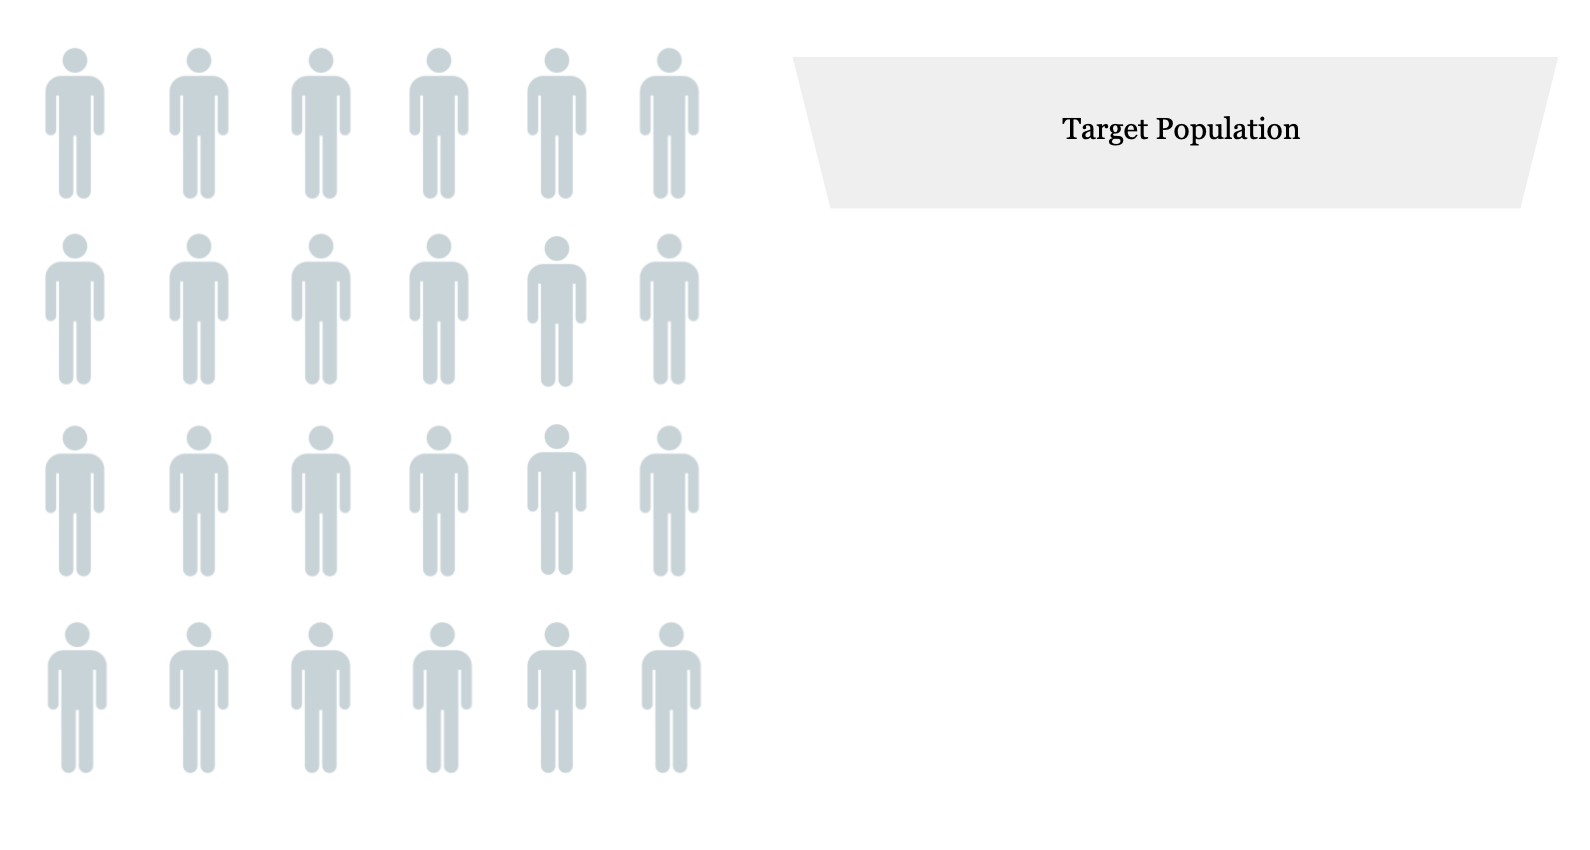
\includegraphics[width=100mm,scale=1]{targetpop.png}

\end{frame}

\begin{frame}{Eligibility}

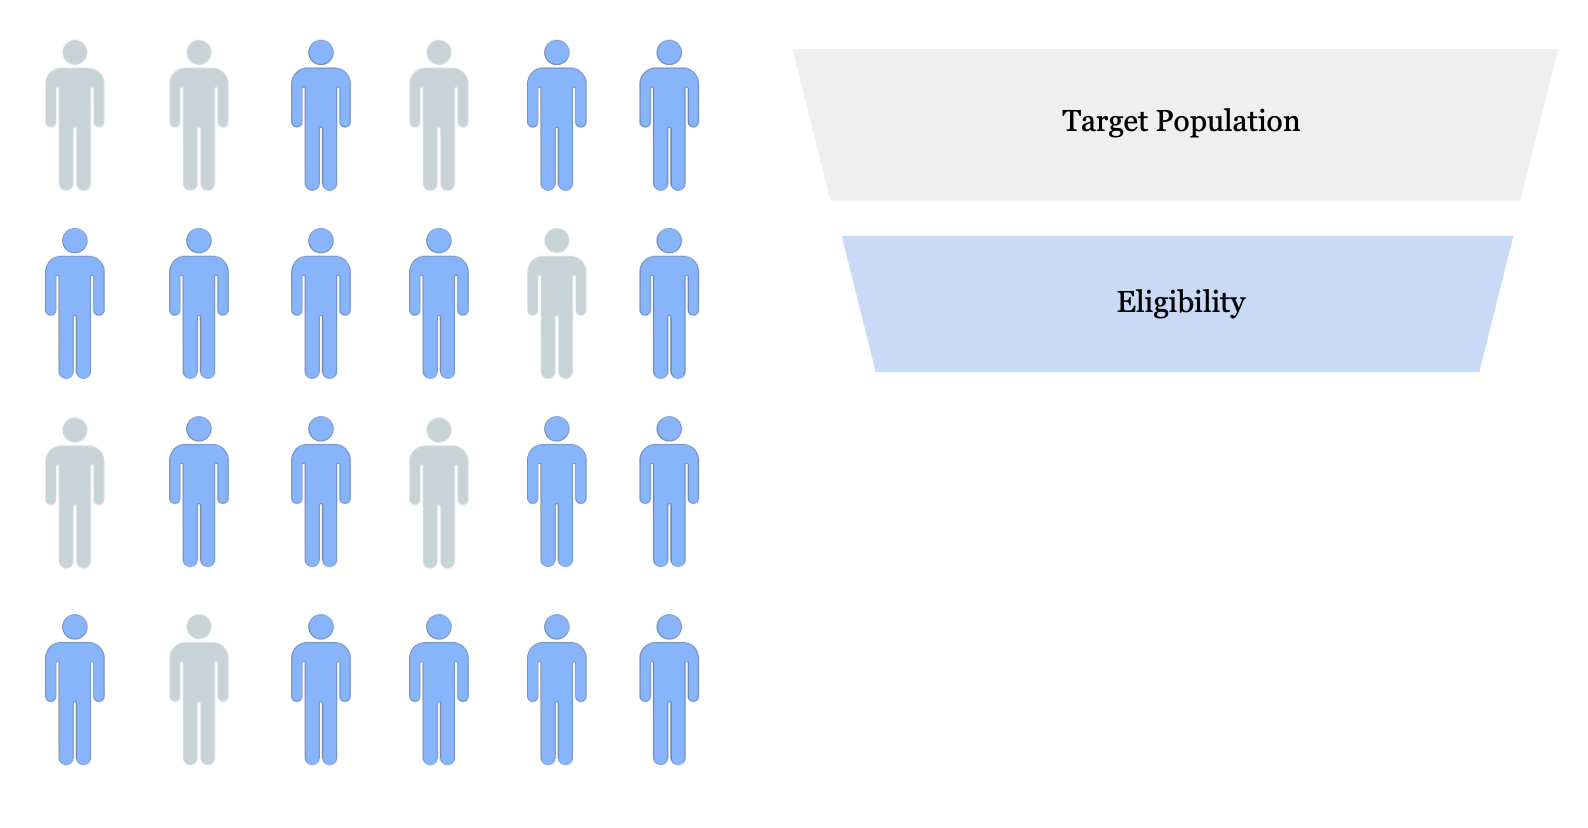
\includegraphics[width=100mm,scale=1]{eligibility.png}

\end{frame}

\begin{frame}{Enrollment}

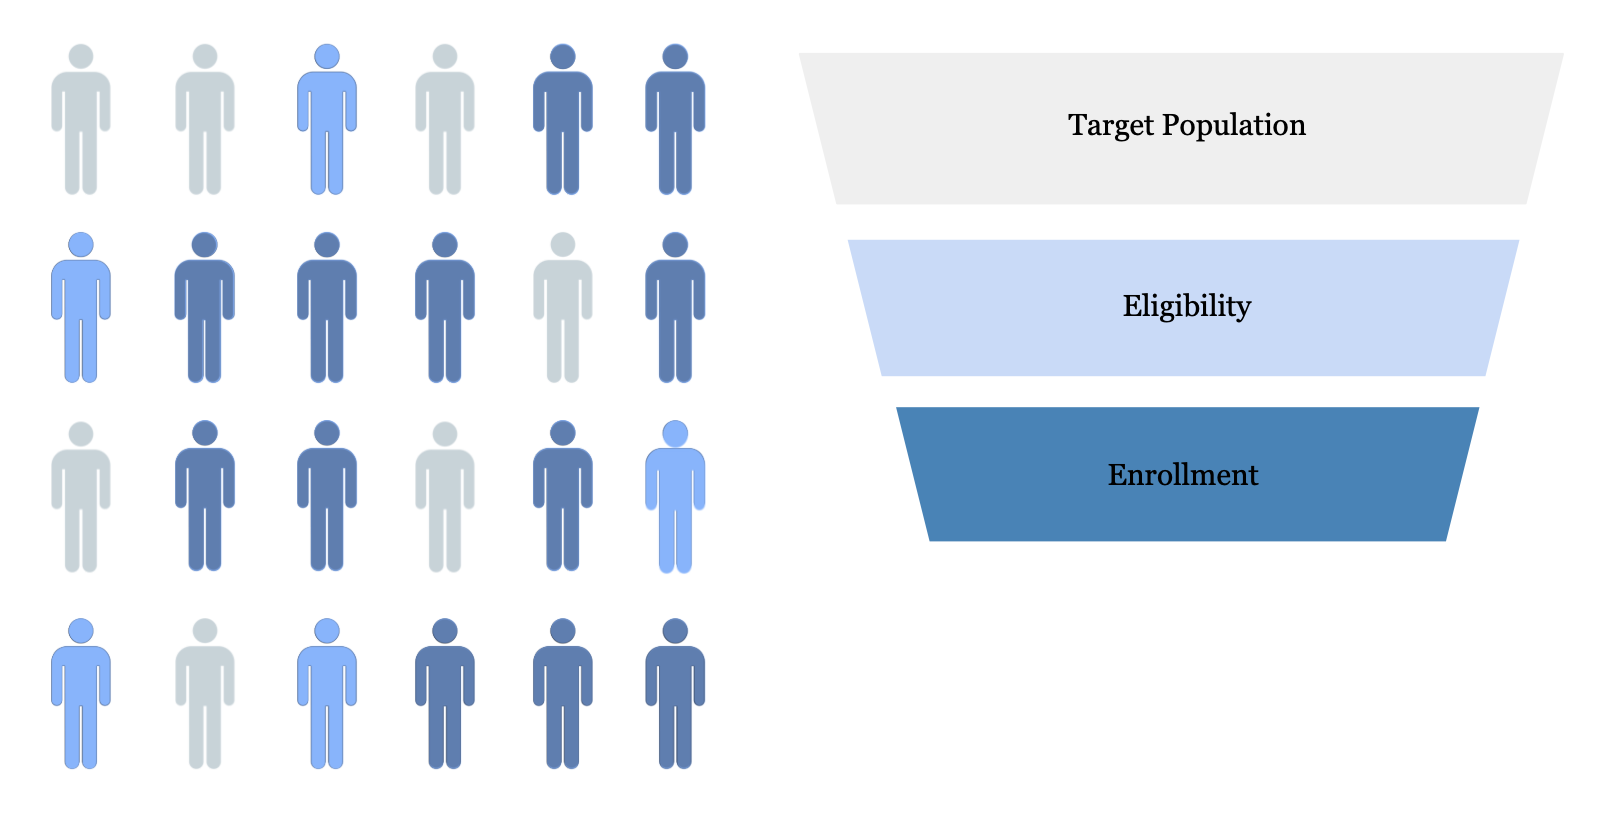
\includegraphics[width=100mm,scale=1]{enrollment.png}


\end{frame}

\begin{frame}{Randomization}

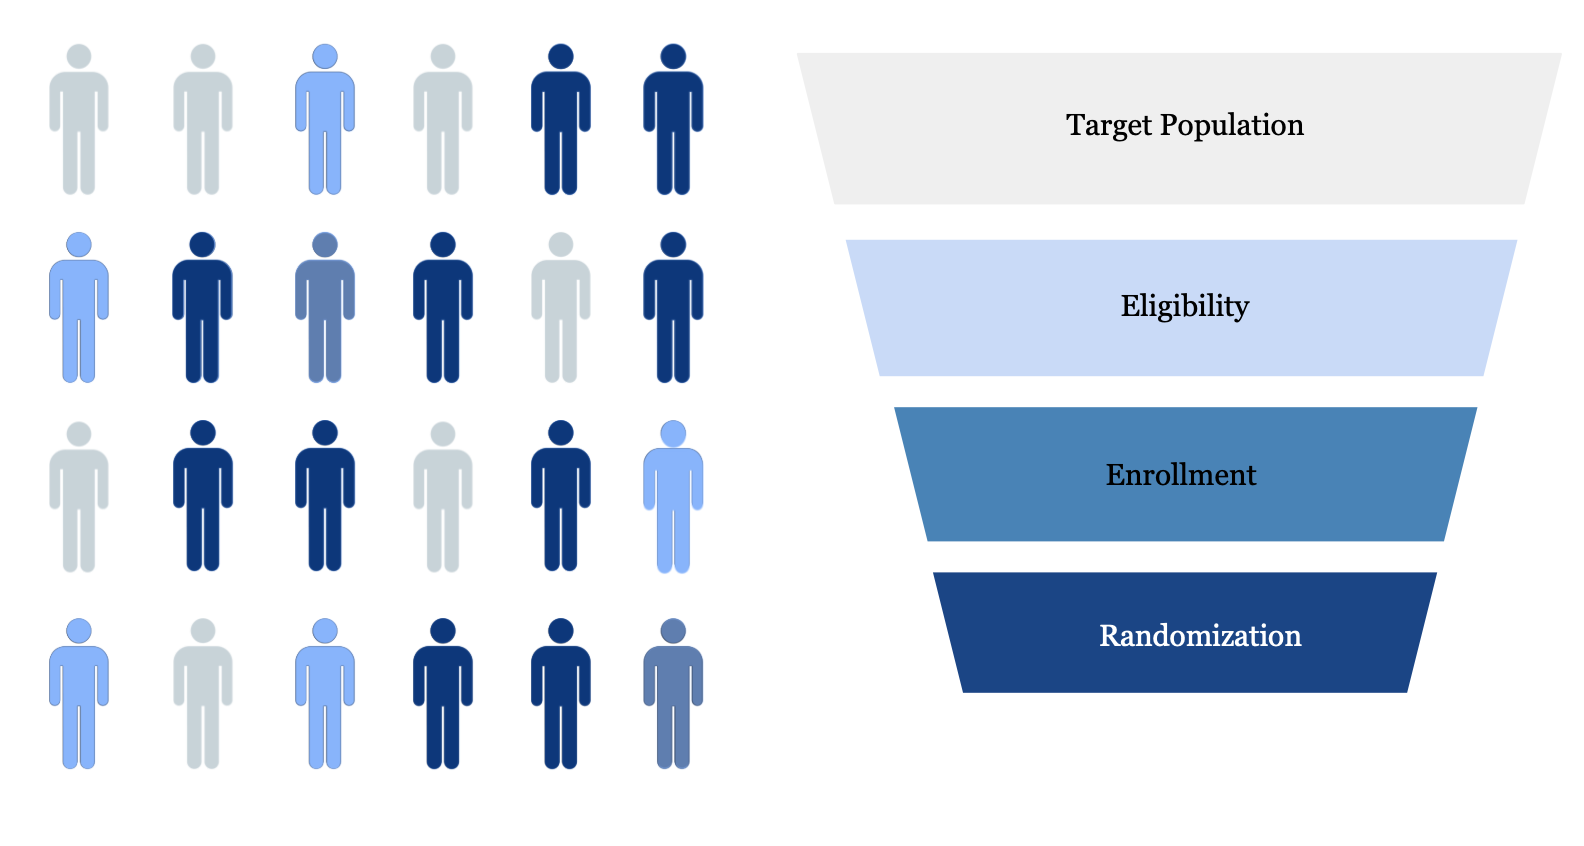
\includegraphics[width=100mm,scale=1]{randomization.png}

\end{frame}

\begin{frame}{Statistical Analysis}

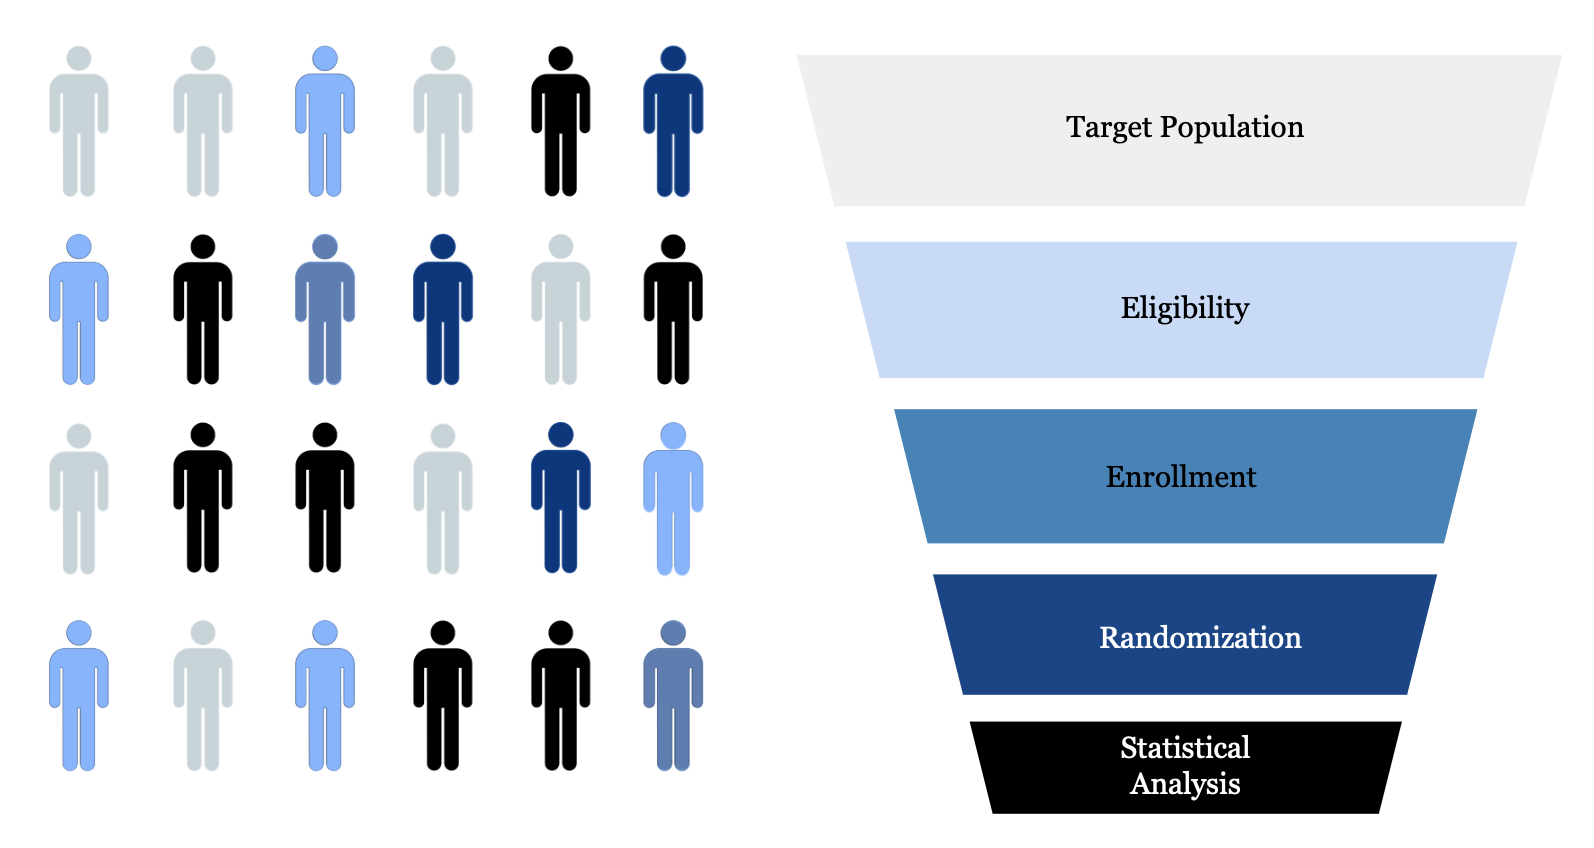
\includegraphics[width=100mm,scale=1]{statanal.png}

\end{frame}


\begin{frame}{Patient Leakage}

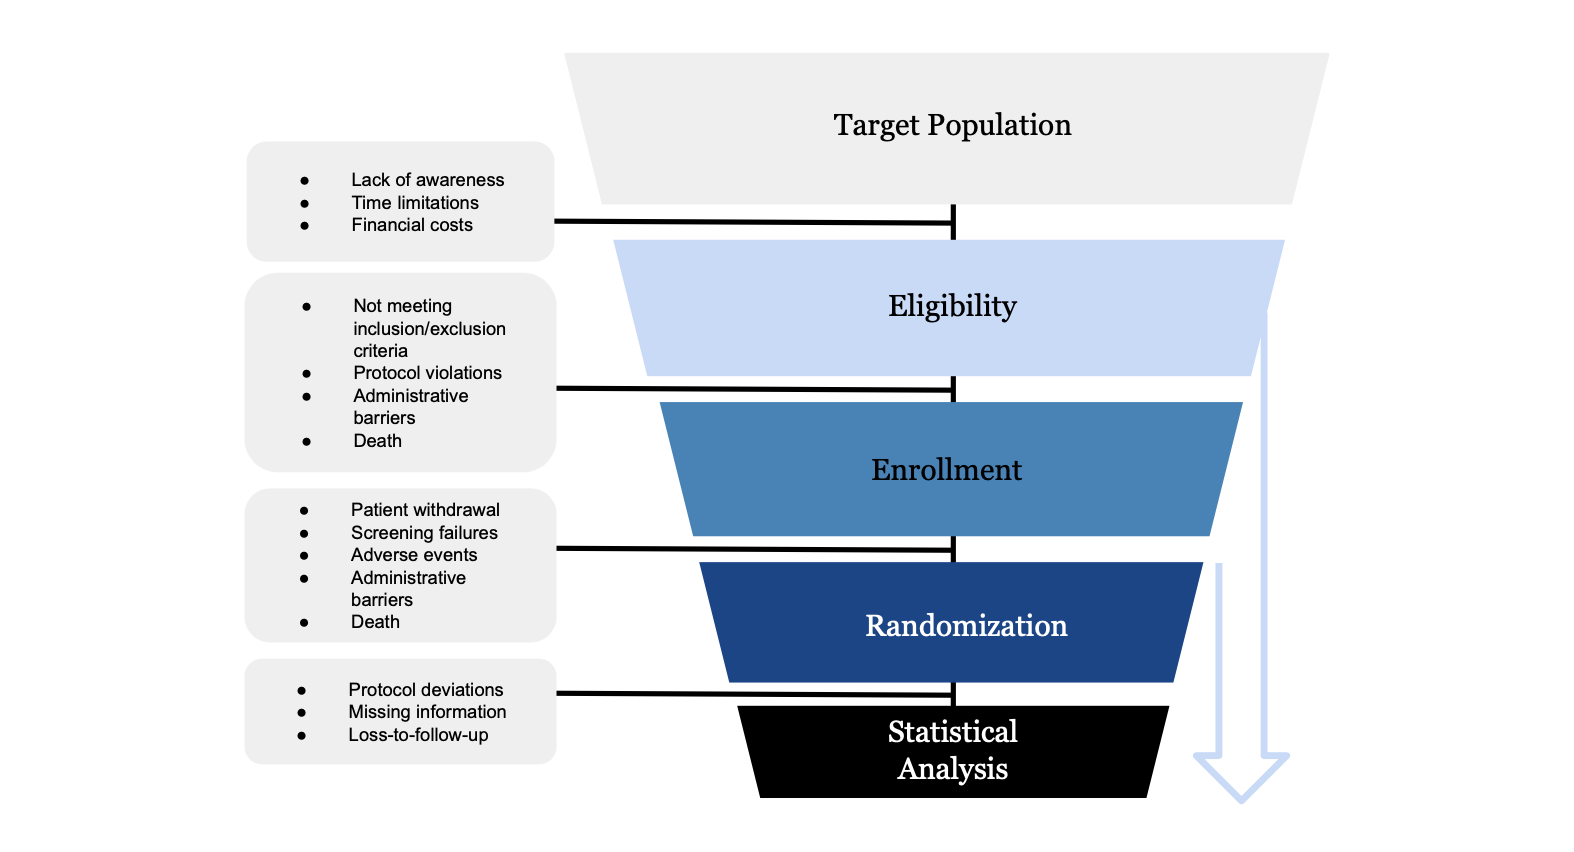
\includegraphics[width=100mm,scale=1]{attrition.png}

\end{frame}


\begin{frame}{Definitions}

\begin{itemize}
\item \textbf{Recruitment rate} = Per time-unit \citep{piantadosi2024clinical}
\begin{align*}
\lambda = \frac{\Delta C}{\Delta T} = \frac{C_1 - C_0}{T_1 - T_0} = \frac{C_1}{T_1}
\end{align*}

\item \textbf{Accrual} = Cumulative Recruitment
\item \textbf{Aleatory uncertainty}: randomness inherent and unpredictable
\item \textbf{Epistemic uncertainty}: arises from limited knowledge about parameters



\end{itemize}


\end{frame}

\begin{frame}[shrink = 5]{Models for Counts}
\textbf{Recruitment} in unit of time (t=1):
\begin{table}[h!]
\centering
\resizebox{\textwidth}{!}{
\begin{tabular}{cccccc}
 \textbf{Methods} & \textbf{Counts} & \textbf{Expectation} & \textbf{Variance} & \textbf{Aleatory} & \textbf{Epistemic} \\
\hline
\hline
Expectation & $C = \lambda$ & $\lambda $ & 0 & No & No \\
Poisson & $C \sim$ Po $(\lambda )$ & $\lambda $ & $\lambda $ & Yes & No \\
Poisson - Gamma & $C \sim Po (\Lambda )$; $\Lambda \sim G(\alpha,\beta)$ & $\frac{\alpha}{\beta}$ & $\frac{\alpha(\beta+1)}{\beta^2}$ & Yes & Yes \\
\end{tabular}
}
\end{table}

\textbf{Accrual} for time t [0,t]:
\begin{table}[h!]
\centering
\resizebox{\textwidth}{!}{
\begin{tabular}{cccccc}
 \textbf{Methods} & \textbf{Counts} & \textbf{Expectation} & \textbf{Variance} & \textbf{Aleatory} & \textbf{Epistemic} \\
\hline
\hline
Expectation & $C(t) = \lambda  t$ & $\lambda  t$ & 0 & No & No \\
Poisson & $C(t) \sim Po (\lambda  t)$ & $\lambda  t$ & $\lambda  t$ & Yes & No \\
Poisson - Gamma & $C(t) \sim Po (\Lambda  t)$; $\Lambda \sim G(\alpha,\beta)$ & $t\frac{\alpha}{\beta}$ & $t\frac{\alpha(\beta+t)}{\beta^2}$ & Yes & Yes \\
\end{tabular}
}
\end{table}

\end{frame}

\begin{frame}{Multicenter Trial on Palliation in Terminal Esophageal Cancer}

Example from \cite{carter2004application}:
\begin{itemize}
\item Recruitment Rate $\lambda = \frac{Counts}{Time} = 0.591$ per day
\item Time $t = 550$ days
\end{itemize}

\end{frame}


\begin{frame}{Multicenter Trial on Palliation in Terminal Esophageal Cancer}

Example from \cite{carter2004application}:
\begin{itemize}
\item Recruitment Rate $\lambda = \frac{Counts}{Time} = 0.591$ per day
\item Time $t = 550$ days
\item Models for Counts:
	\begin{itemize}
	\item \textbf{Expectation}: $EC(t) = \lambda t = 0.591 \cdot 550 = 325$
	\item \textbf{Poisson}: $C(t) \sim Po(\lambda t)$
	\end{itemize}
\end{itemize}

\end{frame}




\begin{frame}{Accrual at time point $t$}
\begin{itemize}
\item \textbf{Expectation}: $EC(t) = E\underbrace{(C +\ldots + C)}_{t \ \text{times}} = t E C = \lambda t$
\item \textbf{Poisson}: $\underbrace{Po (\lambda) +\ldots +Po (\lambda)}_{t \ \text{times}} = Po (\lambda t)$
% mention this is infinitely divisible property of poisson
\end{itemize}
\end{frame}


\begin{frame}{Accrual of 1 study}

\begin{figure}

\begin{knitrout}
\definecolor{shadecolor}{rgb}{0.969, 0.969, 0.969}\color{fgcolor}
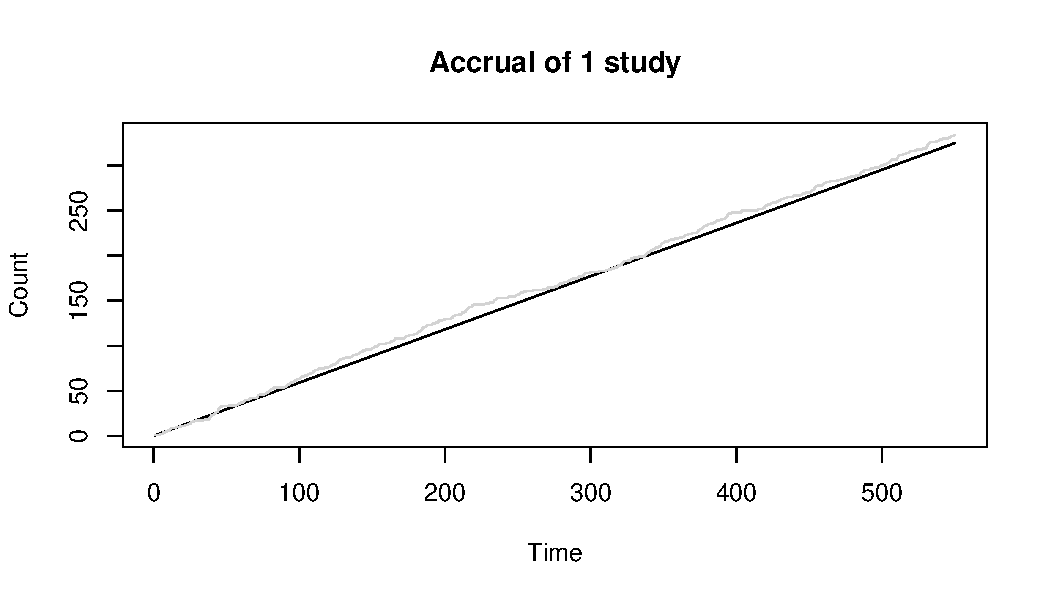
\includegraphics[width=\maxwidth]{figures/figunnamed-chunk-2-1} 
\end{knitrout}
 
\end{figure}


\end{frame}

\begin{frame}{Accrual of 2 studies}

\begin{figure}

\begin{knitrout}
\definecolor{shadecolor}{rgb}{0.969, 0.969, 0.969}\color{fgcolor}
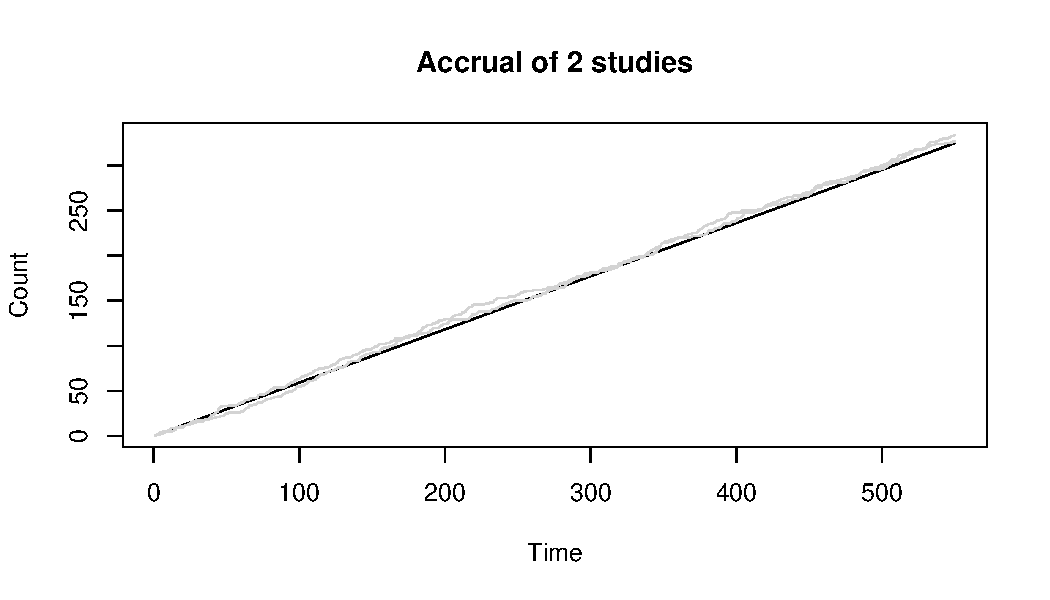
\includegraphics[width=\maxwidth]{figures/figunnamed-chunk-3-1} 
\end{knitrout}
  
\end{figure}


\end{frame}

\begin{frame}{Accrual of 100 studies}

\begin{figure}
\begin{knitrout}
\definecolor{shadecolor}{rgb}{0.969, 0.969, 0.969}\color{fgcolor}
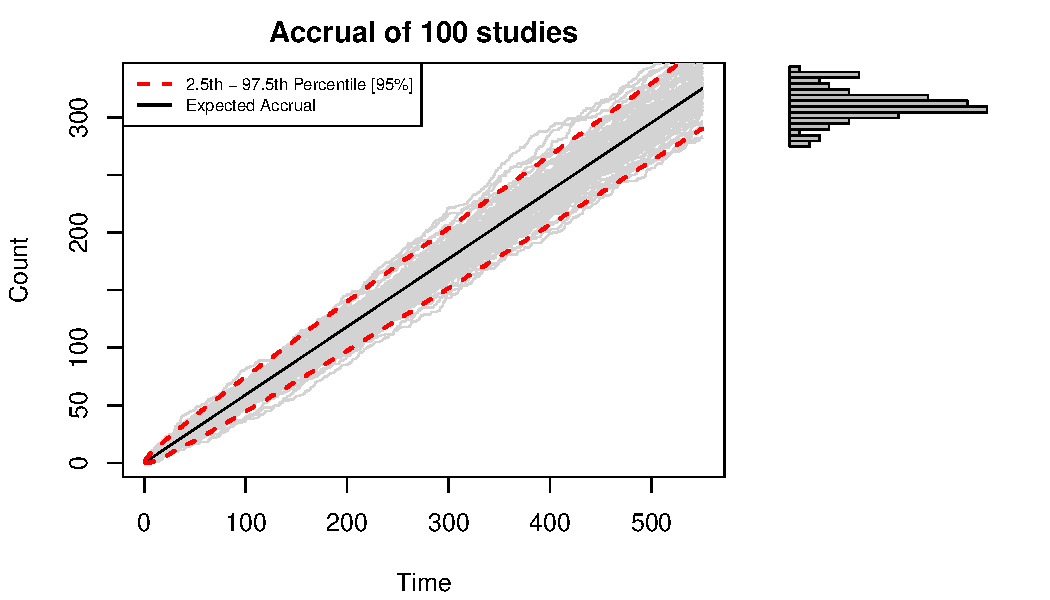
\includegraphics[width=\maxwidth]{figures/figunnamed-chunk-4-1} 
\end{knitrout}

\end{figure}

\end{frame}



\begin{frame}{Poisson's uncertainty bands}


\begin{figure}
\begin{knitrout}
\definecolor{shadecolor}{rgb}{0.969, 0.969, 0.969}\color{fgcolor}
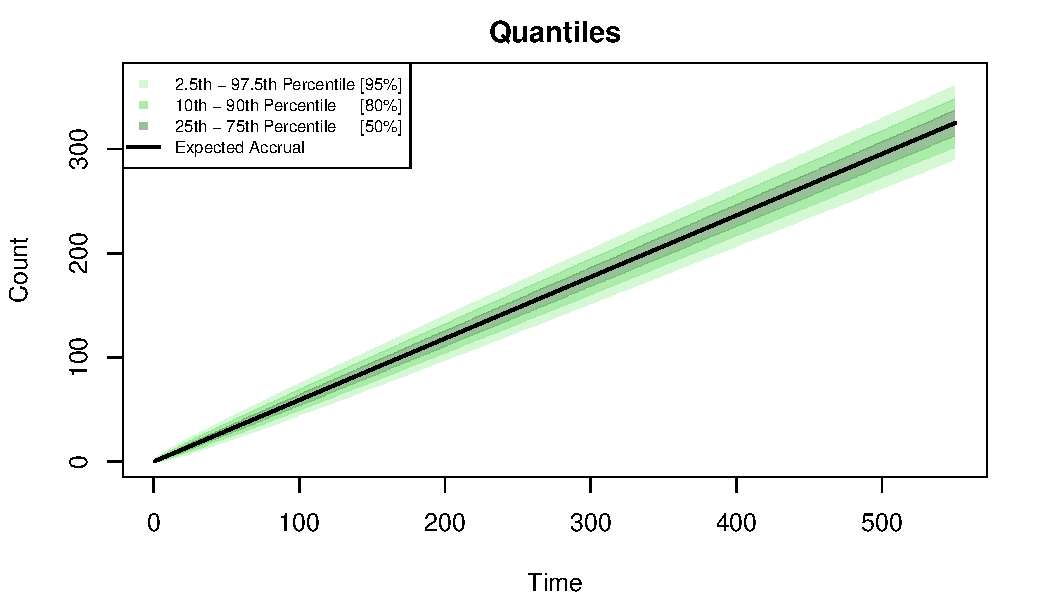
\includegraphics[width=\maxwidth]{figures/figunnamed-chunk-5-1} 
\end{knitrout}
\end{figure}

\end{frame}



\begin{frame}{Poisson's exact PMF at time point $t=550$ with $\lambda = 0.591$}
\begin{figure}
\begin{knitrout}
\definecolor{shadecolor}{rgb}{0.969, 0.969, 0.969}\color{fgcolor}
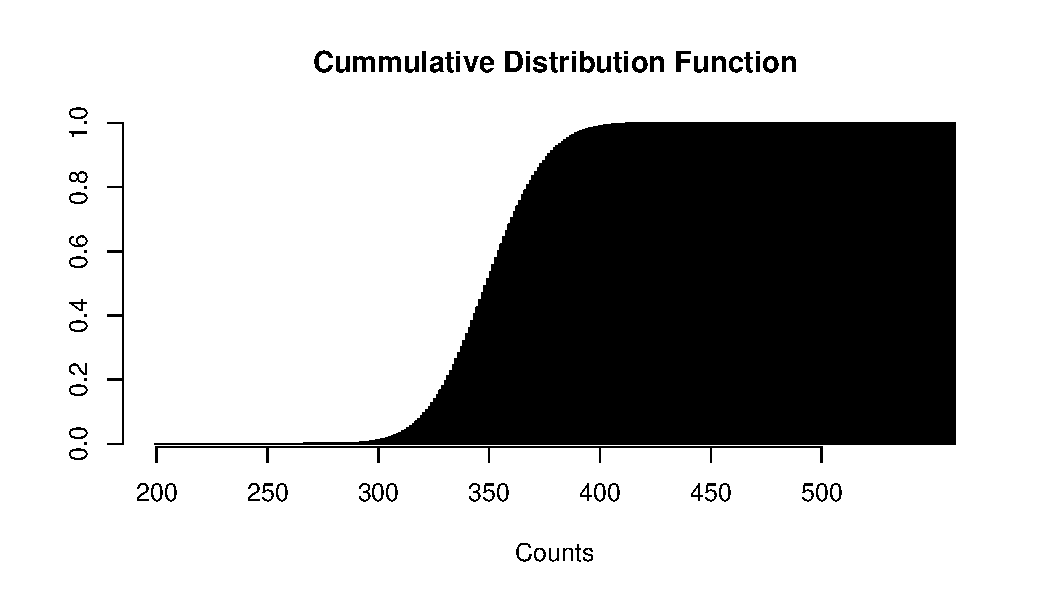
\includegraphics[width=\maxwidth]{figures/figunnamed-chunk-6-1} 
\end{knitrout}
  \caption{Poisson Distribution of Counts: This bar plot represents the probability mass function (PMF) of counts ranging from 200 to 500, using a Poisson distribution with a rate parameter $\lambda = 0.591$ based on 550 time periods.}
  \label{fig:2_3}
\end{figure}
\end{frame}

\begin{frame}{Poisson's exact CDF at time point $t=550$ with $\lambda = 0.591$}

\begin{figure}
\begin{knitrout}
\definecolor{shadecolor}{rgb}{0.969, 0.969, 0.969}\color{fgcolor}
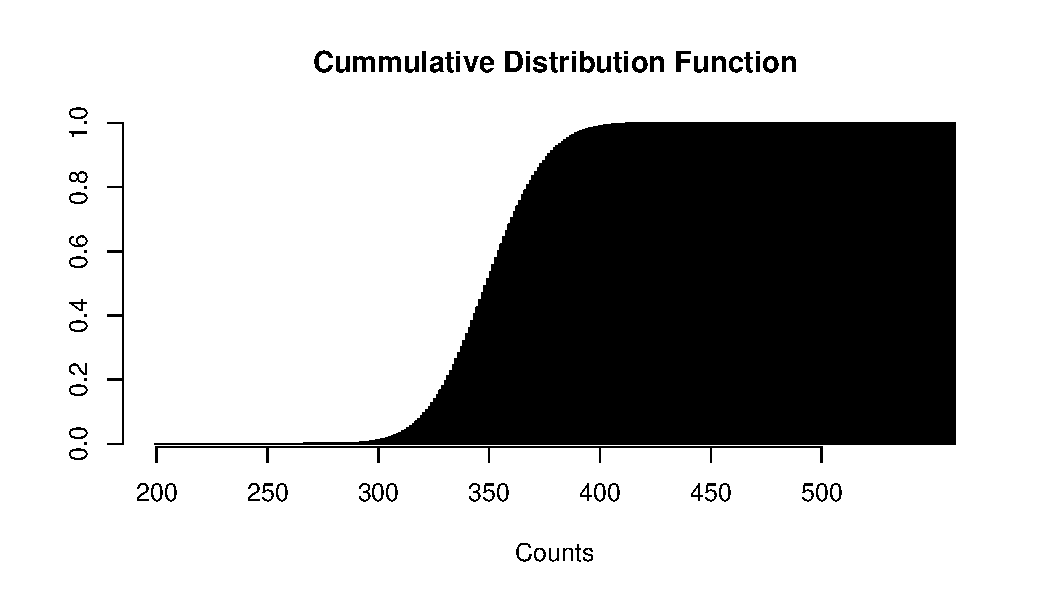
\includegraphics[width=\maxwidth]{figures/figunnamed-chunk-7-1} 
\end{knitrout}
  \caption{Cumulative Distribution of Poisson-Distributed Counts: The plot illustrates the cumulative probability distribution for counts within the range of 200 to 500, using a Poisson distribution with a rate parameter $\lambda = 0.591$ adjusted for 550 time periods.}
  \label{fig:2_4}
\end{figure}
\end{frame}




\begin{frame}{Multicenter Trial on Palliation in Terminal Esophageal Cancer}
Example from \cite{carter2004application}:
\begin{itemize}
\item Recruitment Rate $\lambda = \frac{Counts}{Time} = 0.591$ per day
\item Time $t = 550$ days
\item Models for Counts:
	\begin{itemize}
	\item \textbf{Poisson - Gamma}: $C(t) \sim Po (\Lambda t)$; $\Lambda \sim G(\alpha,\beta)$
		\begin{itemize}
		\item $\alpha = 325$
		\item $\beta = 548$
		\item $E \Lambda = \frac{\alpha}{\beta} = 0.591 = \lambda$
		\end{itemize}
	\end{itemize}
\end{itemize}
\end{frame}

\begin{frame}[shrink = 5]{Negative binomial derived from Poisson-Gamma model (t=1)}

Let $C(t)|\Lambda \sim Po(\Lambda t)$ and $\Lambda \sim G(\alpha,\beta)$
\begin{align*}
p(c)&=\int^\infty_0 p(c|\lambda) p(\lambda) d\lambda\\
&=\int^\infty_0 \frac{(\lambda t)^c\exp(-\lambda t)}{c!}\Bigg[(\lambda t)^{\alpha-1}\exp(-\beta\lambda t)\frac{\beta^\alpha}{\Gamma(\alpha)}\Bigg]d\lambda\\
&=\frac{\beta^\alpha t^c \Gamma(\alpha+c)}{c!\Gamma(\alpha) (\beta+t)^{\alpha+c}}\underbrace{\int^\infty_0 \frac{(\beta+t)^{\alpha+c}}{\Gamma(\alpha+c)} \lambda^{\alpha+c-1}\exp(-(\beta+t)\lambda)d\lambda}_{=1}\\
&=\binom{\alpha+c-1}{\alpha-1}\Bigg (\frac{t}{\beta+t}\Bigg)^{c} \Bigg(\frac{\beta}{\beta+t}\Bigg)^{\alpha}, \\
C(t)|\Lambda\sim NBin \Bigg(\alpha, \frac{\beta}{\beta+t}\Bigg)
\end{align*}
% talk here about interpretations (from report)
\end{frame}


\begin{frame}{Expectation and Variance}
Using the expressions of iterated expectation and variance \citep{held2014applied}

\begin{align*}
E(C(t)) &= E_{\Lambda}[E_{C(t)} (C(t)|\Lambda)] = E_{\Lambda}[\Lambda t] = t\alpha/\beta
\end{align*}

\begin{align*}
Var(C(t)) &= Var_{\Lambda}[E_{C(t)} (C(t)|\Lambda)] + E_{\Lambda}[Var_{C(t)}(C(t)|\Lambda)]\\
&=Var_{\Lambda}[\Lambda t] + E_{\Lambda}[\Lambda t] \\
&=t^2\alpha/\beta^2 + t\alpha/\beta = \frac{t \alpha(\beta+t)}{\beta^2}
\end{align*}
\end{frame}

\begin{frame}{Gamma Prior}
$\Lambda \sim G(\alpha,\beta)$
\begin{knitrout}
\definecolor{shadecolor}{rgb}{0.969, 0.969, 0.969}\color{fgcolor}
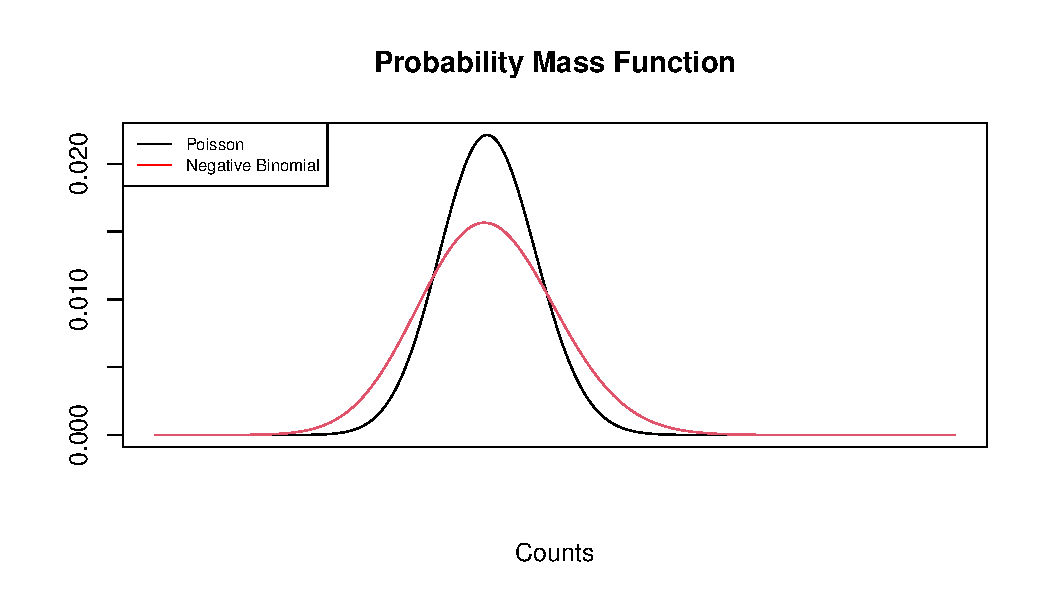
\includegraphics[width=\maxwidth]{figures/figunnamed-chunk-8-1} 
\end{knitrout}

\end{frame}


\begin{frame}{Comparison between Poisson and Poisson - Gamma}
\begin{figure}
\begin{knitrout}
\definecolor{shadecolor}{rgb}{0.969, 0.969, 0.969}\color{fgcolor}
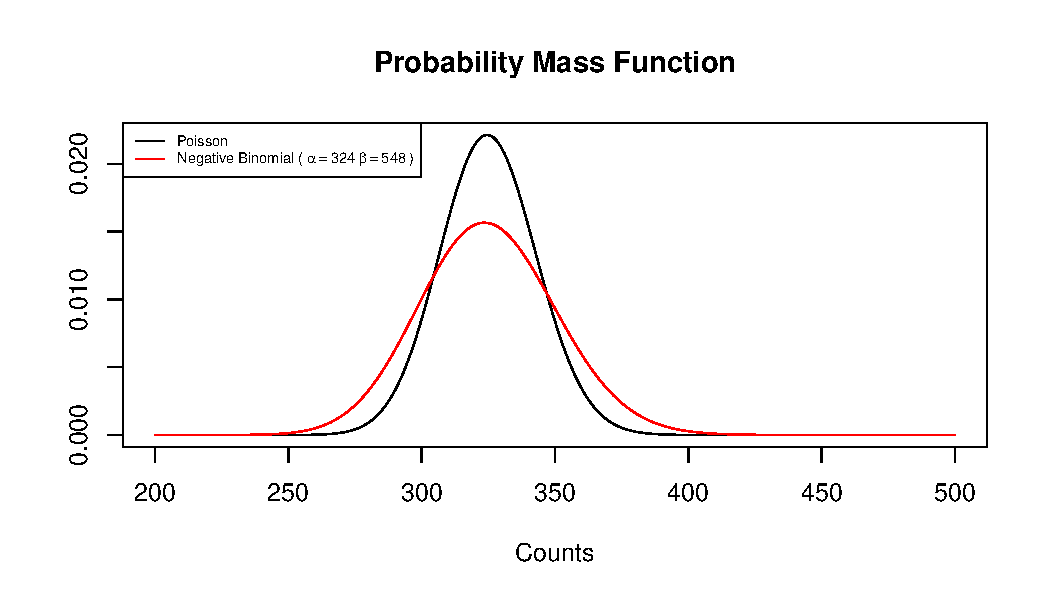
\includegraphics[width=\maxwidth]{figures/figunnamed-chunk-9-1} 
\end{knitrout}
  \caption{Comparison of Probability Mass Function (PMF) between Poisson distribution with $\lambda = 0.591$ and Negative Binomial with $\alpha = 324$ and $\mu = 0.591$.}
  \label{fig:2_6}
\end{figure}
\end{frame}


\begin{frame}{Comparison between Poisson and Poisson - Gamma}

\begin{figure}
\begin{knitrout}
\definecolor{shadecolor}{rgb}{0.969, 0.969, 0.969}\color{fgcolor}
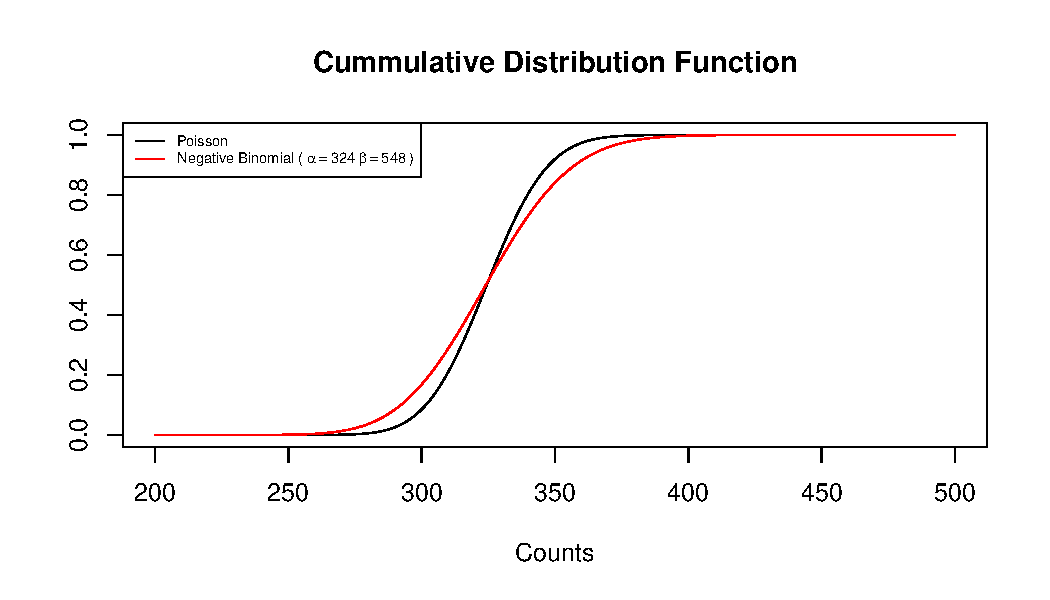
\includegraphics[width=\maxwidth]{figures/figunnamed-chunk-10-1} 
\end{knitrout}
  \caption{Comparison of Cummulative Distribution Function (CDF) between Poisson distribution with $\lambda = 0.591$ and Negative Binomial with $\alpha = 324$ and $\mu = 0.591$.}
  \label{fig:2_7}
\end{figure}

\end{frame}

\begin{frame}{Sensitivity Analysis}


\end{frame}


\begin{frame}{Sensitivity Analysis}
\begin{knitrout}
\definecolor{shadecolor}{rgb}{0.969, 0.969, 0.969}\color{fgcolor}
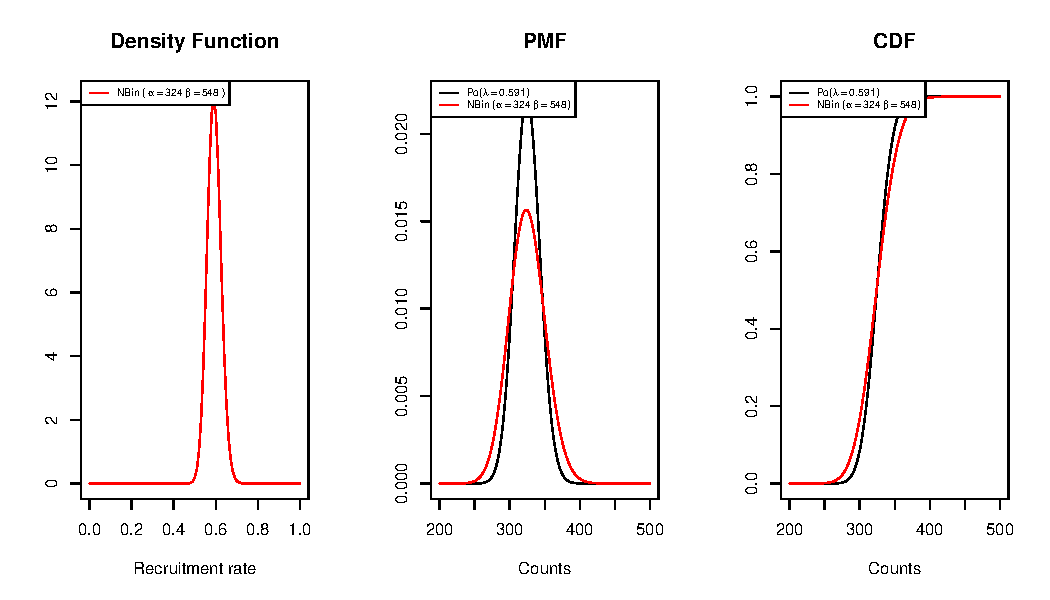
\includegraphics[width=\maxwidth]{figures/figunnamed-chunk-11-1} 
\end{knitrout}

\end{frame}


\begin{frame}{Sensitivity Analysis}
\begin{knitrout}
\definecolor{shadecolor}{rgb}{0.969, 0.969, 0.969}\color{fgcolor}
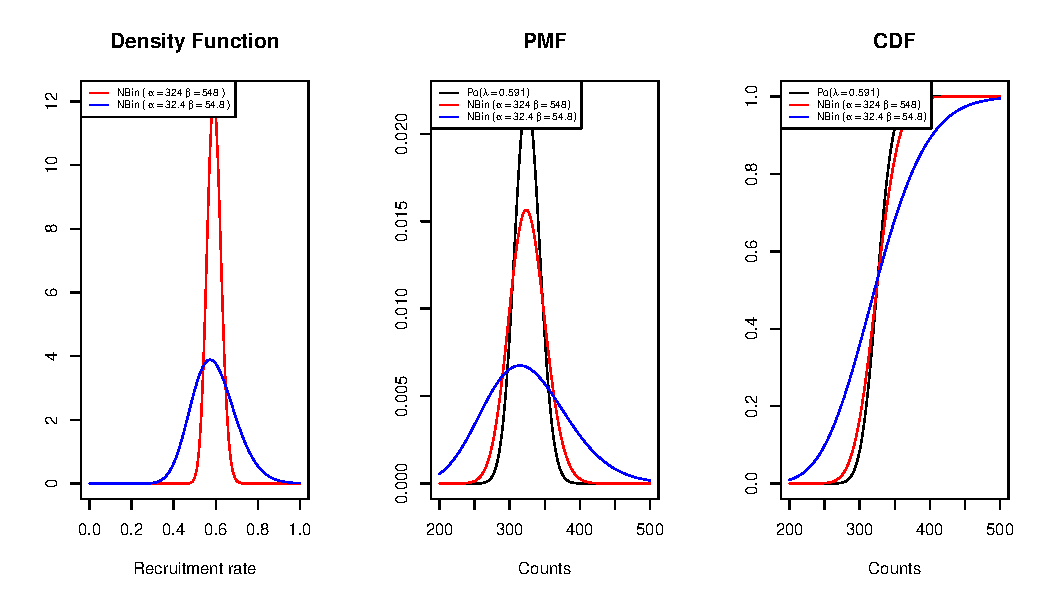
\includegraphics[width=\maxwidth]{figures/figunnamed-chunk-12-1} 
\end{knitrout}

\end{frame}



\begin{frame}{Sensitivity Analysis}
\begin{knitrout}
\definecolor{shadecolor}{rgb}{0.969, 0.969, 0.969}\color{fgcolor}
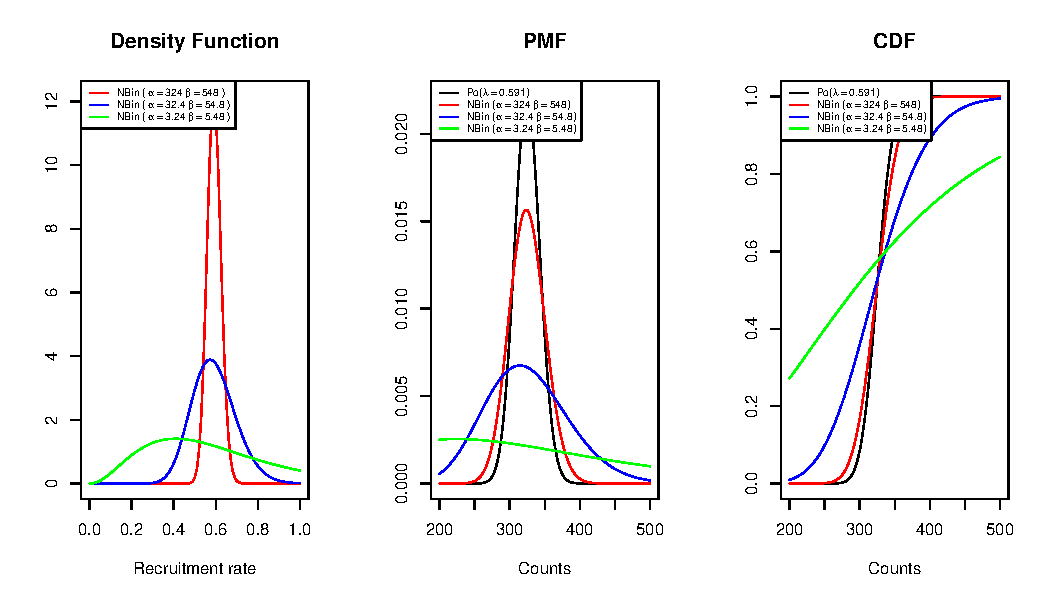
\includegraphics[width=\maxwidth]{figures/figunnamed-chunk-13-1} 
\end{knitrout}

\end{frame}



\begin{frame}[shrink = 5]{Models for Counts}
\textbf{Recruitment} in unit of time (t=1):
\begin{table}[h!]
\centering
\resizebox{\textwidth}{!}{
\begin{tabular}{cccccc}
 \textbf{Methods} & \textbf{Counts} & \textbf{Expectation} & \textbf{Variance} & \textbf{Aleatory} & \textbf{Epistemic} \\
\hline
\hline
Expectation & $C = \lambda$ & $\lambda $ & 0 & No & No \\
Poisson & $C \sim$ Po $(\lambda )$ & $\lambda $ & $\lambda $ & Yes & No \\
Poisson - Gamma & $C \sim Po (\Lambda )$; $\Lambda \sim G(\alpha,\beta)$ & $\frac{\alpha}{\beta}$ & $\frac{\alpha(\beta+1)}{\beta^2}$ & Yes & Yes \\
\end{tabular}
}
\end{table}

\textbf{Accrual} for time t [0,t]:
\begin{table}[h!]
\centering
\resizebox{\textwidth}{!}{
\begin{tabular}{cccccc}
 \textbf{Methods} & \textbf{Counts} & \textbf{Expectation} & \textbf{Variance} & \textbf{Aleatory} & \textbf{Epistemic} \\
\hline
\hline
Expectation & $C(t) = \lambda  t$ & $\lambda  t$ & 0 & No & No \\
Poisson & $C(t) \sim Po (\lambda  t)$ & $\lambda  t$ & $\lambda  t$ & Yes & No \\
Poisson - Gamma & $C(t) \sim Po (\Lambda  t)$; $\Lambda \sim G(\alpha,\beta)$ & $t\frac{\alpha}{\beta}$ & $t\frac{\alpha(\beta+t)}{\beta^2}$ & Yes & Yes \\
\end{tabular}
}
\end{table}

\end{frame}


\begin{frame}{Summary}
\begin{itemize}
\item Extension of Carter's approach based on MC simulations
\item Exact models for \textbf{counts}
\item Unified notation
\item Visualization of study accrual and uncertainty bands 
\item Sensitivity analysis
\end{itemize}

\end{frame}


\begin{frame}{Next steps}
\begin{itemize}
\item Compare exact models for counts to those provided by \cite{carter2004application}
\item Models for \textbf{time} 
	\begin{itemize}
	\item Exact models
	\item Compare them to those provided by Carter
	\end{itemize}
\item Shiny App
\item Apply theoretical results to dataset
\end{itemize}

\end{frame}

\begin{frame}{References}
  \small
  \bibliographystyle{apalike}
\bibliography{illustration}
\end{frame}


\begin{frame}{Thank you for your attention}

\end{frame}

%\appendix
%% Possible backup slides...

%% chapter division is accomplished with:
%% \part{Appendix}

\end{document}
